%!TEX root = ../../report.tex

\subsection{Noise} % (fold)
\label{ssub:noise}


``To generate irregular procedural textures, we need an irregular primitive function, usually called noise" \cite{Ebert2002}. It's a pseudorandom function that gave the goal to break the monotony of a pattern and make it look more random.
Perlin Noise is the most known and used noise function. It was created by Ken Perlin, for the movie Tron 1982 with the aiming to generate natural looking textures.

The psedorandom property is important and a true random function like \emph{white noise} would not do the job. If we generate a texture based on white noise the pattern would change every time it's generated and we would like that the it stays the same, frame after frame. This is achieved with the use of inputs for this functions that with the same input returns always the same output sequence. 

The properties of an ideal \emph{noise} functions are as follows \cite{Ebert2002}:
\begin{itemize}
	\item \emph{noise} is a repeatable pseudorandom function of its inputs
	\item \emph{noise} has a known range, namely, from -1 to 1.
	\item \emph{noise} is band-limited, with a maximum frequency of about 1.
	\item \emph{noise} doesn't exhibit obvious periodicities or regular patterns. Such pseudorandom functions are always periodic, but the period can be made very long and therefore the periodicity is not conspicuous.
	\item \emph{noise} is \emph{stationary} - that is, its statistical character should be translationally invariant
	\item \emph{noise} is \emph{isotropic} - that is, its statistical character should be rotationally invariant
\end{itemize}

With this noise function, it's generated a sequence of values that are interpolated to generate a coherent noise. With the application of \emph{turbulence} that is composition of several layers of this noise with different frequencies and amplitudes forming a coherent noise. This layers are called \emph{Octaves} and the ratio between amplitude and frequency of the layers can be expressed as a constant known as \emph{persistence} \cite{Kelly2008}. With the result we can create a texture that looks natural and with fractal like structure.

\begin{figure}[htbp]
	\centering
	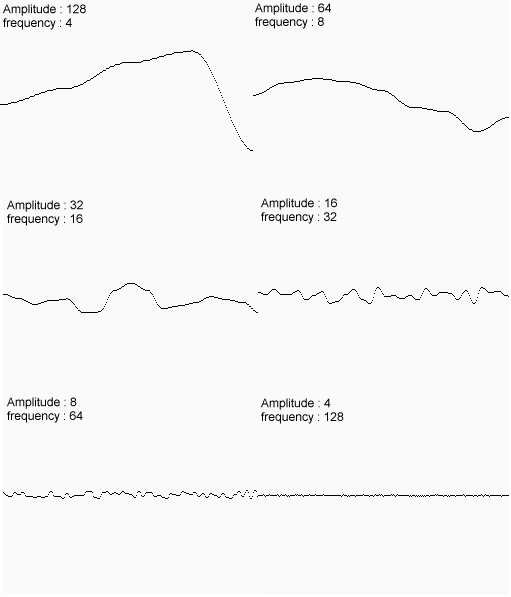
\includegraphics[width=0.55\textwidth]{img/Theory/Perlin_Noise/Merge.png}
	\caption{Different noise functions}
	\label{fig:merge}
\end{figure}

For instance, the Figure~\ref{fig:merge} shows the result of the interpolation over six noise functions with different frequencies and different amplitudes. And the sum of all this functions is the exibithed in the Figure~\ref{fig:noise} \cite{NoisesELIAS}.

\begin{figure}[htbp]
	\centering
	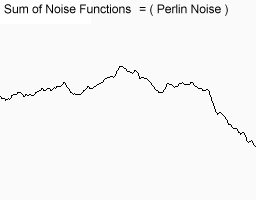
\includegraphics[width=0.55\textwidth]{img/Theory/Perlin_Noise/perlin1.png}
	\caption{``You may even imagine that it looks a little like a mountain range."}
	\label{fig:noise}
\end{figure}

Noise can also be used to generate planes. The method used is the same as the 1D problem but we have to generate a lot more data points that after are interpolated as a plane. This results in noisy images that are often used to model clouds, smoke and other textures with similar visual properties, Figure~\ref{fig:NTextures}. Another application for this technique is the generation of height maps like the one in figure .

\begin{figure}
        \centering
        \begin{subfigure}[b]{0.3\textwidth}
                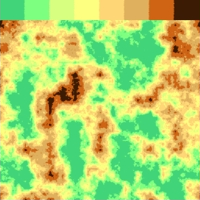
\includegraphics[width=\textwidth]{img/Theory/Perlin_Noise/gradient_discrete.png}
                \label{fig:Fleaf}
        \end{subfigure}%
        ~ %add desired spacing between images, e. g. ~, \quad, \qquad, \hfill etc.
          %(or a blank line to force the subfigure onto a new line)
        \begin{subfigure}[b]{0.3\textwidth}
                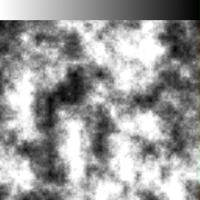
\includegraphics[width=\textwidth]{img/Theory/Perlin_Noise/gradient_grey.png}
                \label{fig:Fbrocoli}
        \end{subfigure}
        ~ %add desired spacing between images, e. g. ~, \quad, \qquad, \hfill etc.
          %(or a blank line to force the subfigure onto a new line)
        \begin{subfigure}[b]{0.3\textwidth}
                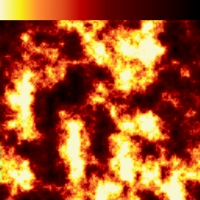
\includegraphics[width=\textwidth]{img/Theory/Perlin_Noise/gradient_fire.png}
                \label{fig:Fbrocoli}
        \end{subfigure}
        \caption{Gradient mapped textures from \cite{NoisesGAMES}}
        \label{fig:NTextures}
\end{figure}

Another application for Noise planes are with \emph{object placement} on a grid. By creating a noise plane with the same size of the grid, with each cell of the grid corresponding to one pixel of noise, the object placement is done by choosing each object for each cell according to the noise value. Figure~\ref{fig:MyNCity}.
Figure~\ref{fig:NCity} shows a city which the buildings where placed with the use of a noise plane. In this case the noise domain was splitted in three intervals, each one corresponds to one type of building (commercial, industrial or residential). After setting the type for one block, the system randomly chooses one from a set of buildings of that type.

\begin{figure}[htbp]
    \centering
    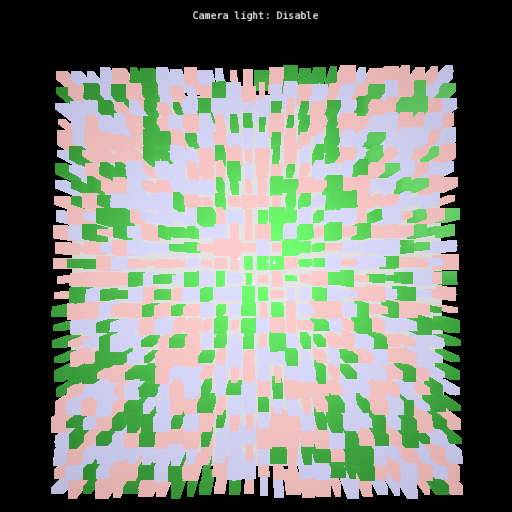
\includegraphics[width=0.55\textwidth]{img/Theory/Perlin_Noise/AppletNoName201501191604.png}
    \caption{Objects Placed following a noise function}
    \label{fig:MyNCity}
\end{figure}

\begin{figure}[htbp]
	\centering
	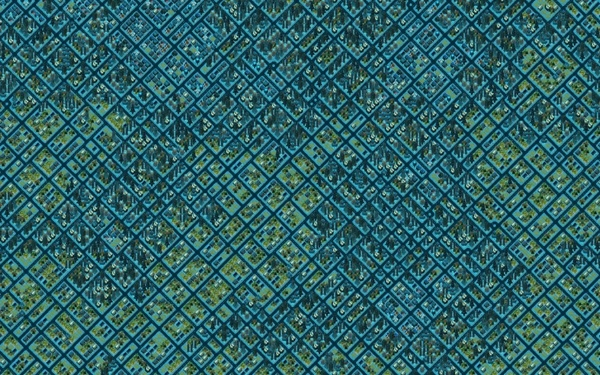
\includegraphics[width=0.55\textwidth]{img/Theory/Perlin_Noise/NoisyCity.jpg}
	\caption{Objects Placed with a noise plane from \cite{NoisesGAMES}}
	\label{fig:NCity}
\end{figure}

% subsubsection noise (end)